Scintillators are widely employed for radiation detection in nuclear physics. Scintillators convert kinetic energy of the incoming particles into light\footnote{The light is made up of photons in the visible energy range.} which can be detected and quantified. Light emission is produced due to the photon de-excitation of scintillating atoms.

Light production is linear in a wide energy range of incoming particles. Scintillators should have good optical properties, such as being transparent to the wavelenght of their own emission and having a refractive index as close as possible to that of glass for optimizing optical coupling with photosensors. Photon emission in scintillators is a statistical process, which means that identical events emmit a different number of photons that follows a Poisson statistics.

Scintillators can be organic and inorganic. Inorganic scintillators normally have a higher atomic number and density, so their light output is higher. For these reasons they are better for gamma-ray spectroscopy. Organic scintillators are generally faster and they are commonly used for beta spectroscopy and neutron detection. This section is focussed on organic scintillators since they are the ones used in the TRITIUM project. 

Organic scintillators are based on a scintillator material dissolved in a base solvent, normally aromatic hydrocarbons as $\ce{C_{18}H_{14}}$, $\ce{C_{24}H_{22}N_{2}O}$ or $\ce{C_{15}H_{11}NO}$ with an average atomic number between 3,5 and 5. The scintillator molecules of organic scintillators have a $\pi$-electron structure. The energy levels of their electrons are commonly ilustrated with a Jablonsky diagram, shown in Figure \ref{fig:JablonskyDiagram}. This diagram shows the fundamental singlet state, $S_{0i}$, where the valence electrons are, the excited singlet states, $S_{jk}$, and the excited triplet states, $T_{lm}$. The energy difference between $S_1$ and $S_0$ states is around $3$ or $4~\eV$ (the visible range). As it is shown in the figure, each energy state is splitted in close sublevels separated around $0.15~\eV$. This fine energy structure is due to excitations of molecular vibrational modes tagged by the second index of the energy states. As the energy levels and sublevels have an energy larger than the termal energy, $0.025~\eV$, non-excited electrons are in the ground state $S_{00}$ at STP\footnote{Standard temperature and pressure conditions}.

\begin{figure}[htbp]
\centering
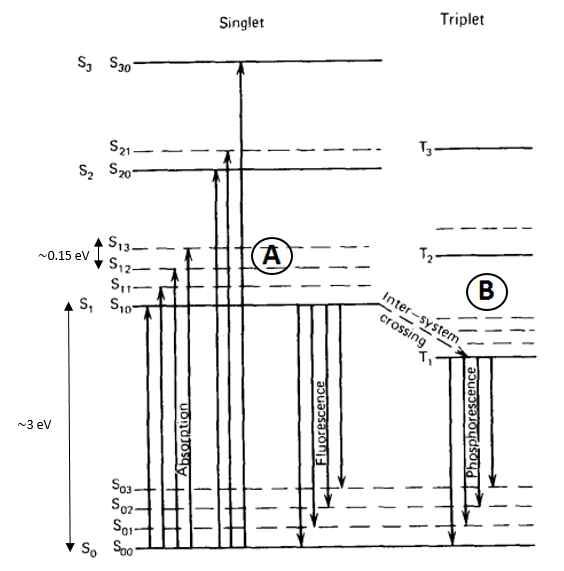
\includegraphics[scale=0.57]{3DesignPrinciples/32Tritium_detector/JablonskyDiagram.png}
\caption{Jablonsky diagram\label{fig:JablonskyDiagram}~\cite{Knoll}.}
\end{figure}

When a particle deposits its kinetic energy in a scintillator, the valence electrons are exited to higher singlet energetic states very fast (times of the order of picoseconds) and are quickly de-excited to the first singlet excited state, $S_{10}$, through non-radiative processes known as internal conversion. These electrons can de-excite to the fundamental single state, $S_{00}$, through three different physical mechanisms:

\begin{enumerate}

\item{} Prompt fluorescence(process A in Figure \ref{fig:JablonskyDiagram}), where the electron in the $S_{10}$ energy level  is de-excited to some sublevel of the ground state $S_{0i}$, emitting a photon. This process happens immediately after the excitation of the scintillator molecules (around tens of nanoseconds after excitation). Each scintillator has a characteristic emission spectrum that defines its response due to the fluorescence mechanism. 

Organic scintillators are practically transparent to their own fluorescense emission because there exist a quenching effect in each de-excitation process by which all emmited  photons by the scintillator have less energy than the excitation energy. This effect is called Stokes shift and it is represented in Figure \ref{fig:StokesShift}.

\begin{figure}[htbp]
\centering
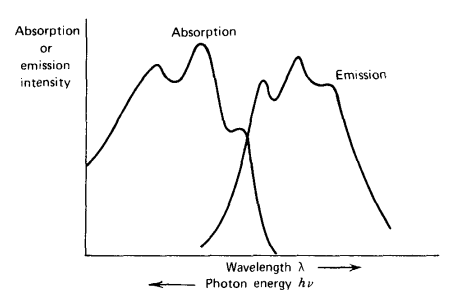
\includegraphics[scale=0.7]{3DesignPrinciples/32Tritium_detector/StokesShift.png}
\caption{Stokes shift\label{fig:StokesShift}~\cite{Knoll}.}
\end{figure}

The intensity of the fluorescence emission in an organic scintillator versus time is the combination of two exponential functions, one associated with the lifetime of the level, $\tau$ (on the order of nanoseconds), and the other associated with the energetic level population, $\tau_1$ (on the order of picoseconds) \cite{Knoll}.

\begin{equation}
I=I_0\left(e^{t/\tau} - e^{t/\tau_1}\right) 
\label{eq:IntensityTimeScintillator}
\end{equation}

\item{} Phosphorescence, where the electron that is in the first single excited state cross to a triple excited state (process B in Figure \ref{fig:JablonskyDiagram}) with a process called "intersystem crossing". This is a metastable state with a longer lifetime than phosphorescence. This process happens around $10^{-3}$ seconds after scintillator excitation.

\item{} Delayed fluorescence, which occurs when an electron is in a triple excited state but its transition to the ground state is forbidden. In this case, the electron interacts with another electron in a similar state, falling to the first singlet state and quickly de-exciting to the ground state. 

\begin{equation}
T_{1} ~+~ T_{1}~ \longrightarrow ~ S_{1} ~+~ S_{0} ~+~ phonons
\label{eq:DelayFluorescence}
\end{equation}

This emission has the same emission spectrum as immediate fluorescence, but with a longer lifetime.
\end{enumerate}
As the prompt fluorescence light produces the scintillator signal, the detector design should optimize its detection and reduce other possible physical mechanisms. One of the most important parameters is the scintillation yield\footnote{The scintillation yield is a way of expressing the efficiency of the scintillator in converting the energy deposited by the particle into photons.}, defined as the the number of photons emitted per unit of absorbed energy. This yield depends on the type of particle and on other mechanisms that do not produce prompt fluorescence, like phosphorescence, delayed fluorescence, or even internal conversion. The scintillator yield is normally quoted by the manufacturer for mips\footnote{The MIP, Minimum Ionized Particles, is a particle that has the speed that generate minimum ionization, that's, for example, electrons with $500~\keV$ or more}.
